\documentclass{article}
\usepackage{graphicx}
\usepackage{caption}
\graphicspath{ {./images/} }
 
\begin{document}
\paragraph{A Look at the Captured Trace}
  \begin{enumerate}
    \item Select the first ICMP echo request message sent by your computer and expand the internet protocol part of the packet int he packet detials window.  What ist he IP address of your computer?
            \begin{itemize}
            \item The IP Address of my computer is: 10.106.0.254
            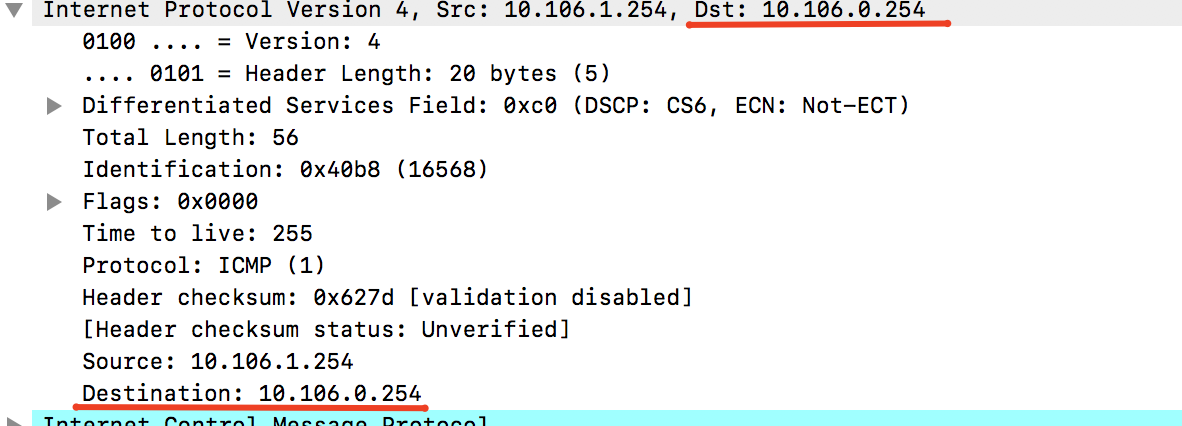
\includegraphics[scale=0.3]{images/IP1.png}
          \end{itemize}

      \item Within the IP packet header, what is the value in the upper layer protocol field?
          \begin{itemize}
            \item The value in the upper layer protocol field is ICMP(1)
            \item 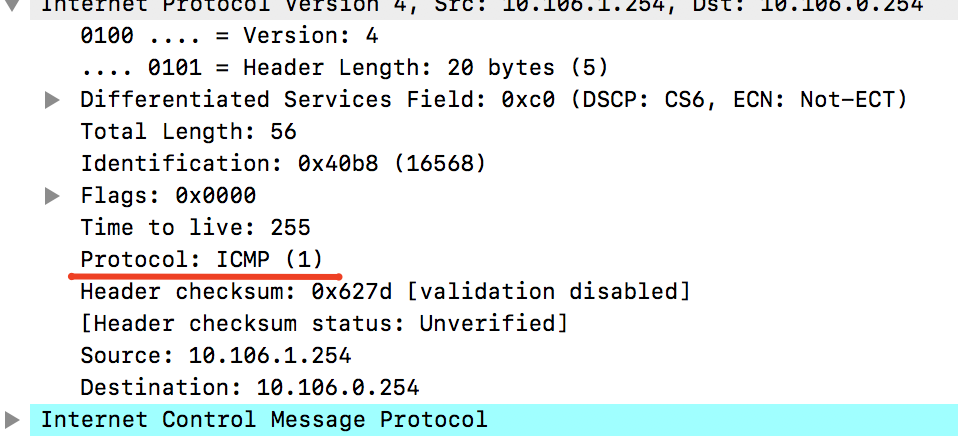
\includegraphics[scale=0.5]{images/IP2.png}
          \end{itemize}

      \item How many bytes are in the ip header?  How many bytes are in the payload of the IP datagram?  Explain how you determined the number of payload bytes.
          \begin{itemize}
            \item Header:
              \begin{itemize}
                \item Size: 20 bytes
                \item 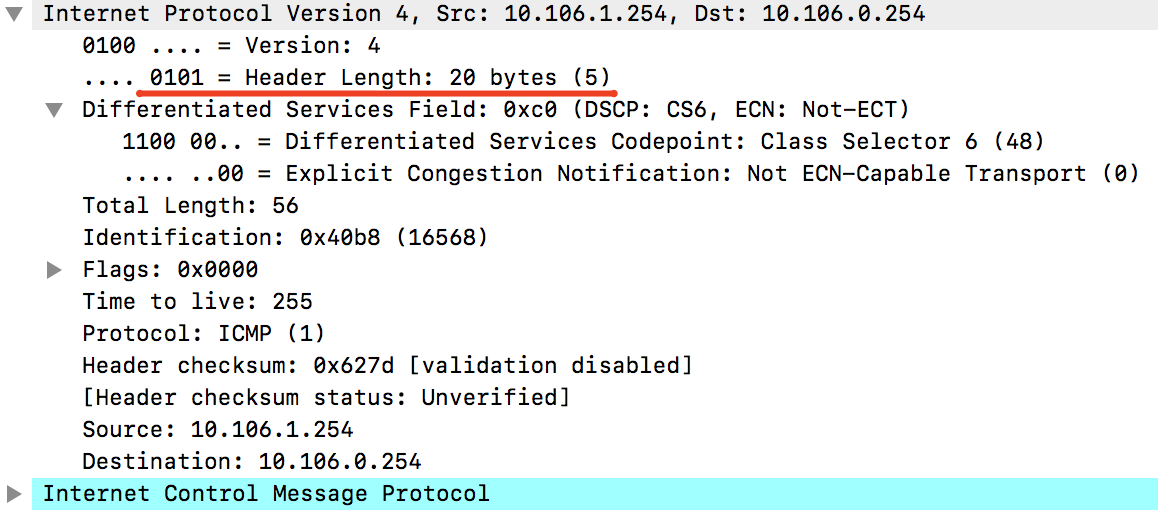
\includegraphics[scale=0.5]{images/IP3.png}
              \end{itemize}
            \item Payload:
              \begin{itemize}
                \item The size of the payload is all of the data in the ICMP excluding the header (56 total - 20 header bytes)
                \item 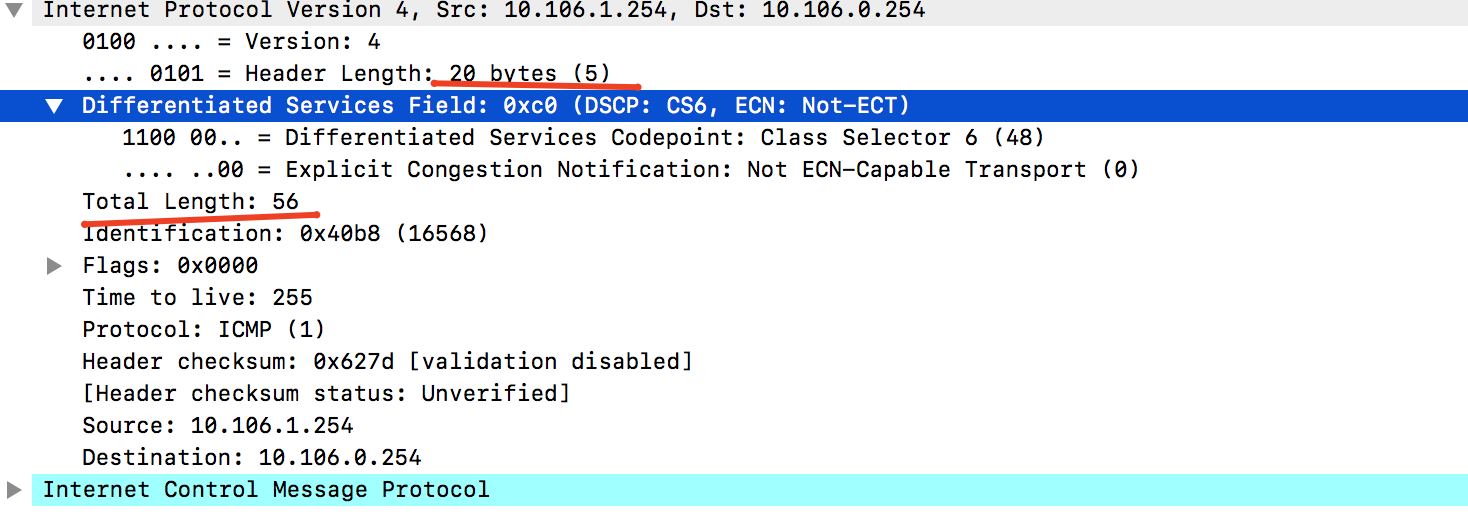
\includegraphics[scale=0.5]{images/IP3b.png}
              \end{itemize}
          \end{itemize}

      \item Has this IP datagram been fragmented?  Explain how you determined whether or not the datagram has been fragmented?
          \begin{itemize}
            \item Wireshark tells us fragmentation has occured if the Fragmentation bit is set, or the Fragmentation offset is greater than 0.  Our fragmentation bit is set to 0 and our fragmentation offset is also set to 0, so our IP Datagram has not been fragmented.
            \item 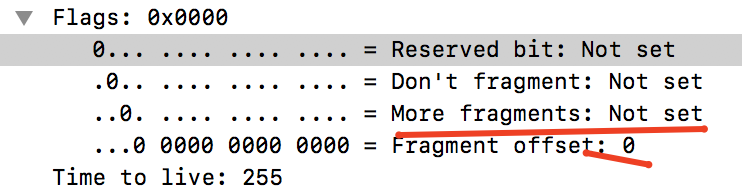
\includegraphics[scale=0.5]{images/IP4.png}
          \end{itemize}

      \item Which fields in the IP datagram always change from one datagram to the next within this series of ICMP messages sent by your computer?
          \begin{itemize}
            \item The TTL field, and the Identification field change from packet to packet.
            \item Packet A:\par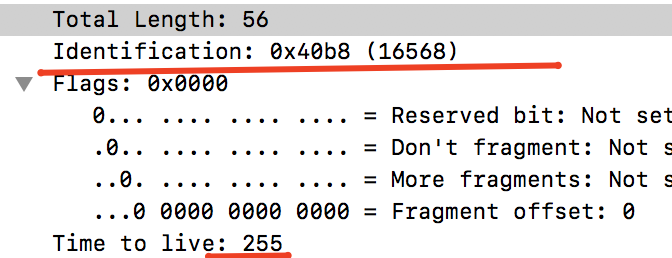
\includegraphics[scale=0.5]{images/IP5a.png}
            \item Packet B:\par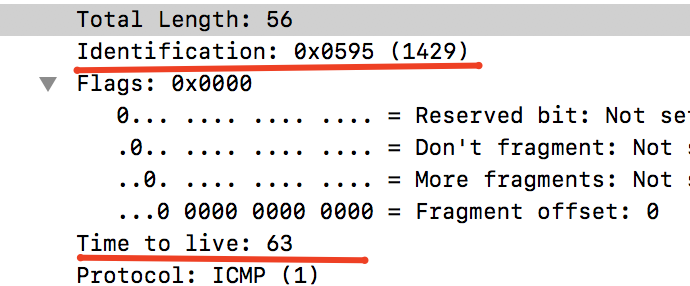
\includegraphics[scale=0.5]{images/IP5b.png}
          \end{itemize}

      \item Which field stays constatn?  Which of the fields must stay constant?  Which fields must change? Why?
          \begin{itemize}
            \item As Stated earlier the fields that change are:
              \begin{itemize}
                \item TTL Field: the TTL field increments as seen earlier, this is how the router communicates.
                \item Identification Field: Every IP Datagram must have a unique identifier
              \end{itemize}
            \item The Fields that remeain constant are:
              \begin{itemize}
                \item The Internet Protocol Version
                \item The Header Length
                \item Src IP
                \item Dst IP
                \item Upper Layer Protocol Field
              \end{itemize}
              
            \item Packet A:\par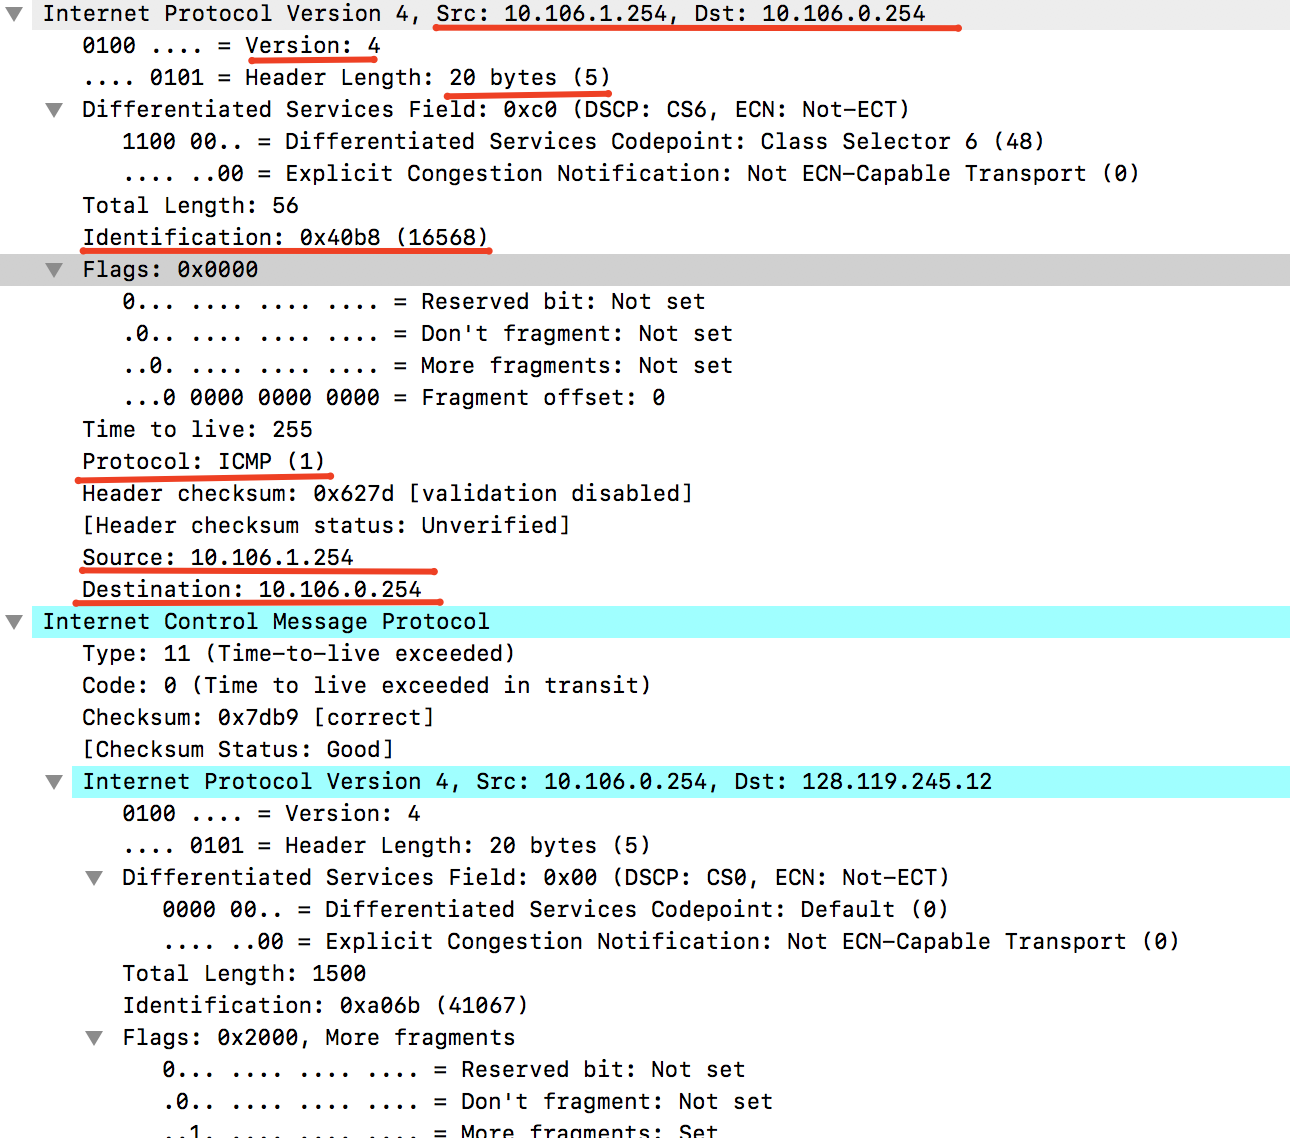
\includegraphics[scale=0.5]{images/IP6a.png}
            \item Packet B:\par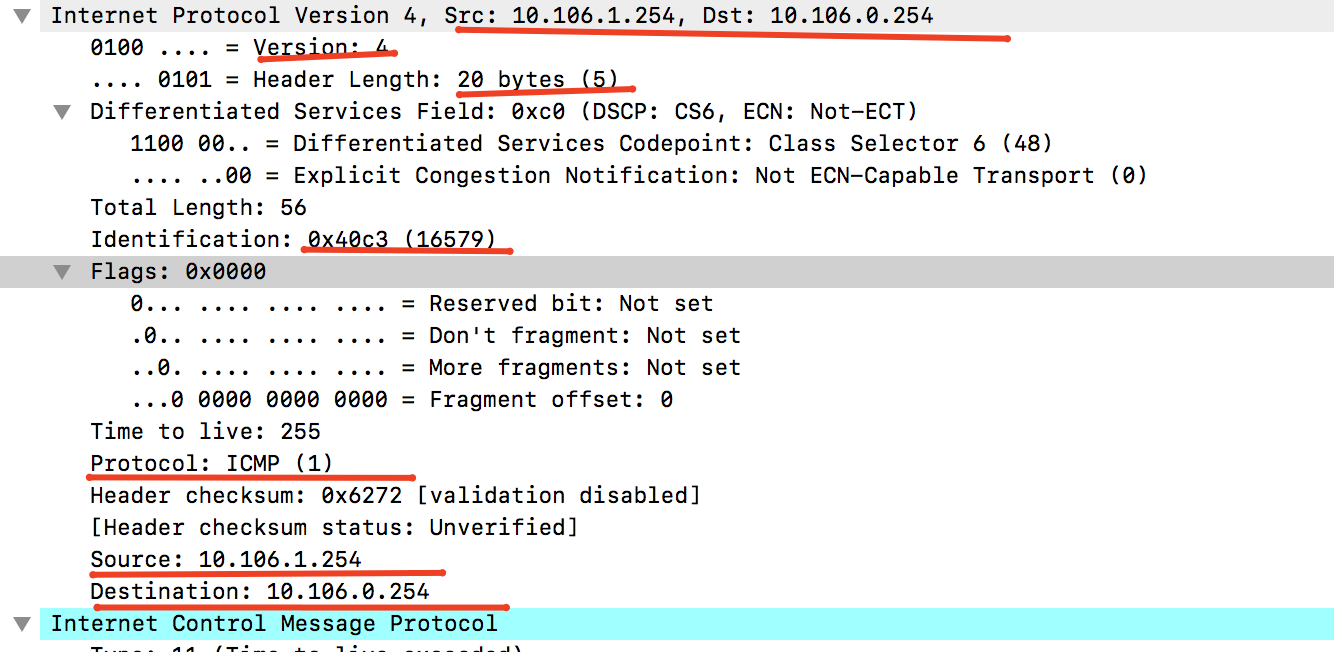
\includegraphics[scale=0.5]{images/IP6b.png}

          \end{itemize}

      \item Describe the pattern you see in the values in the IDentification field of the IP Datagram 
          \begin{itemize}
            \item The Identification fields appear to be increasing in the Internet Protocol Version 4 field, and in the ICMP fields they appear to be decreasing.
          \end{itemize}

      \item What is the value in the Identification field and the TTL field? 
          \begin{itemize}
            \item Identification Field: 0x81e9 
            \item TTL Field 255
            \item 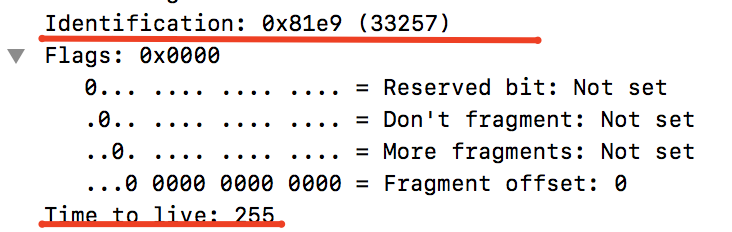
\includegraphics[scale=0.5]{images/IP8.png}
          \end{itemize}

      \item Do these values remain uncahnged for all of the ICMP TTL-exceeded replies sent to your computer by the nearest (first hop) router? Why? 
          \begin{itemize}
            \item The Identification field changes because each packet needs a unique identifier
            \item The TTL remains the same because the first hop router hasn't decremented the TTL field yet.
            \item Packet A:\par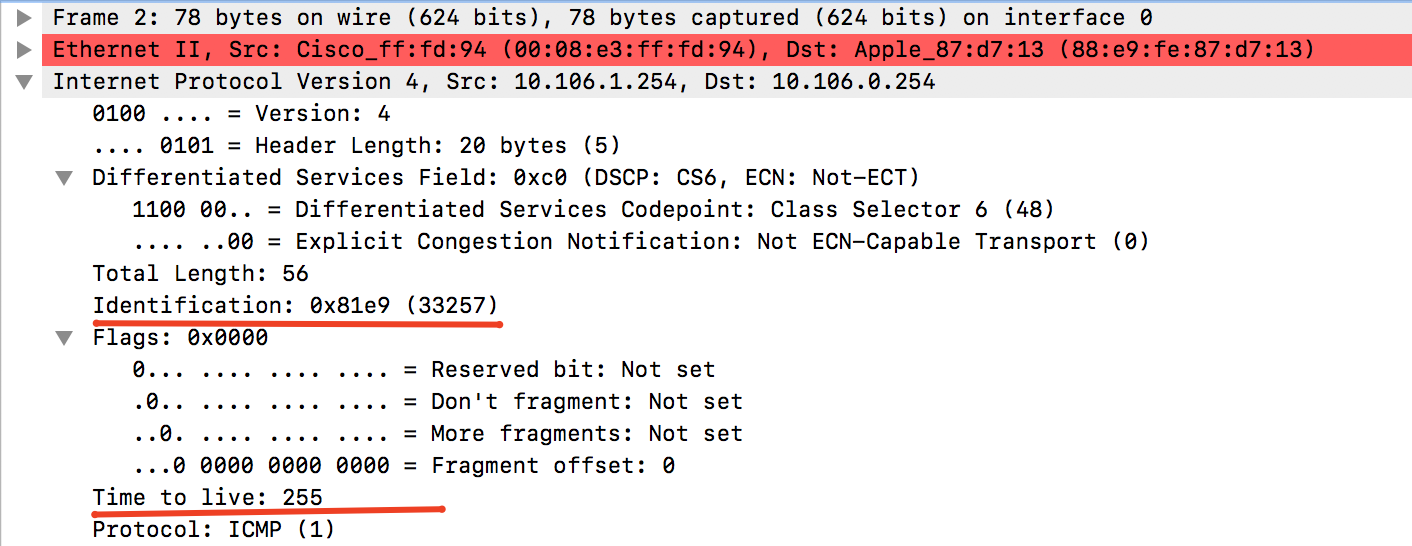
\includegraphics[scale=0.5]{IP9a.png}
            \item Packet B:\par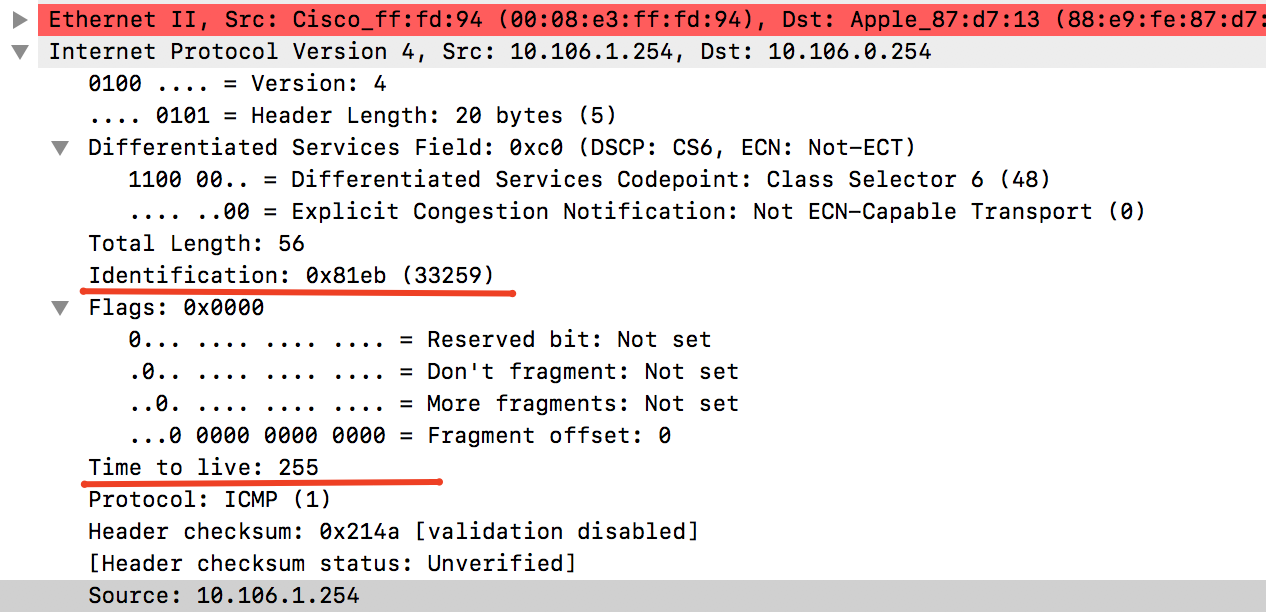
\includegraphics[scale=0.5]{IP9b.png}
          \end{itemize}

      \paragraph{Fragmentation}
      \item Find the first ICMP echo request message that was sent by your computer after you changed the Packet Size in pingplotter to be 2000. 
          \begin{itemize}
            \item Yes, the packet has been fragmented across more than one IP Datagram
            \item 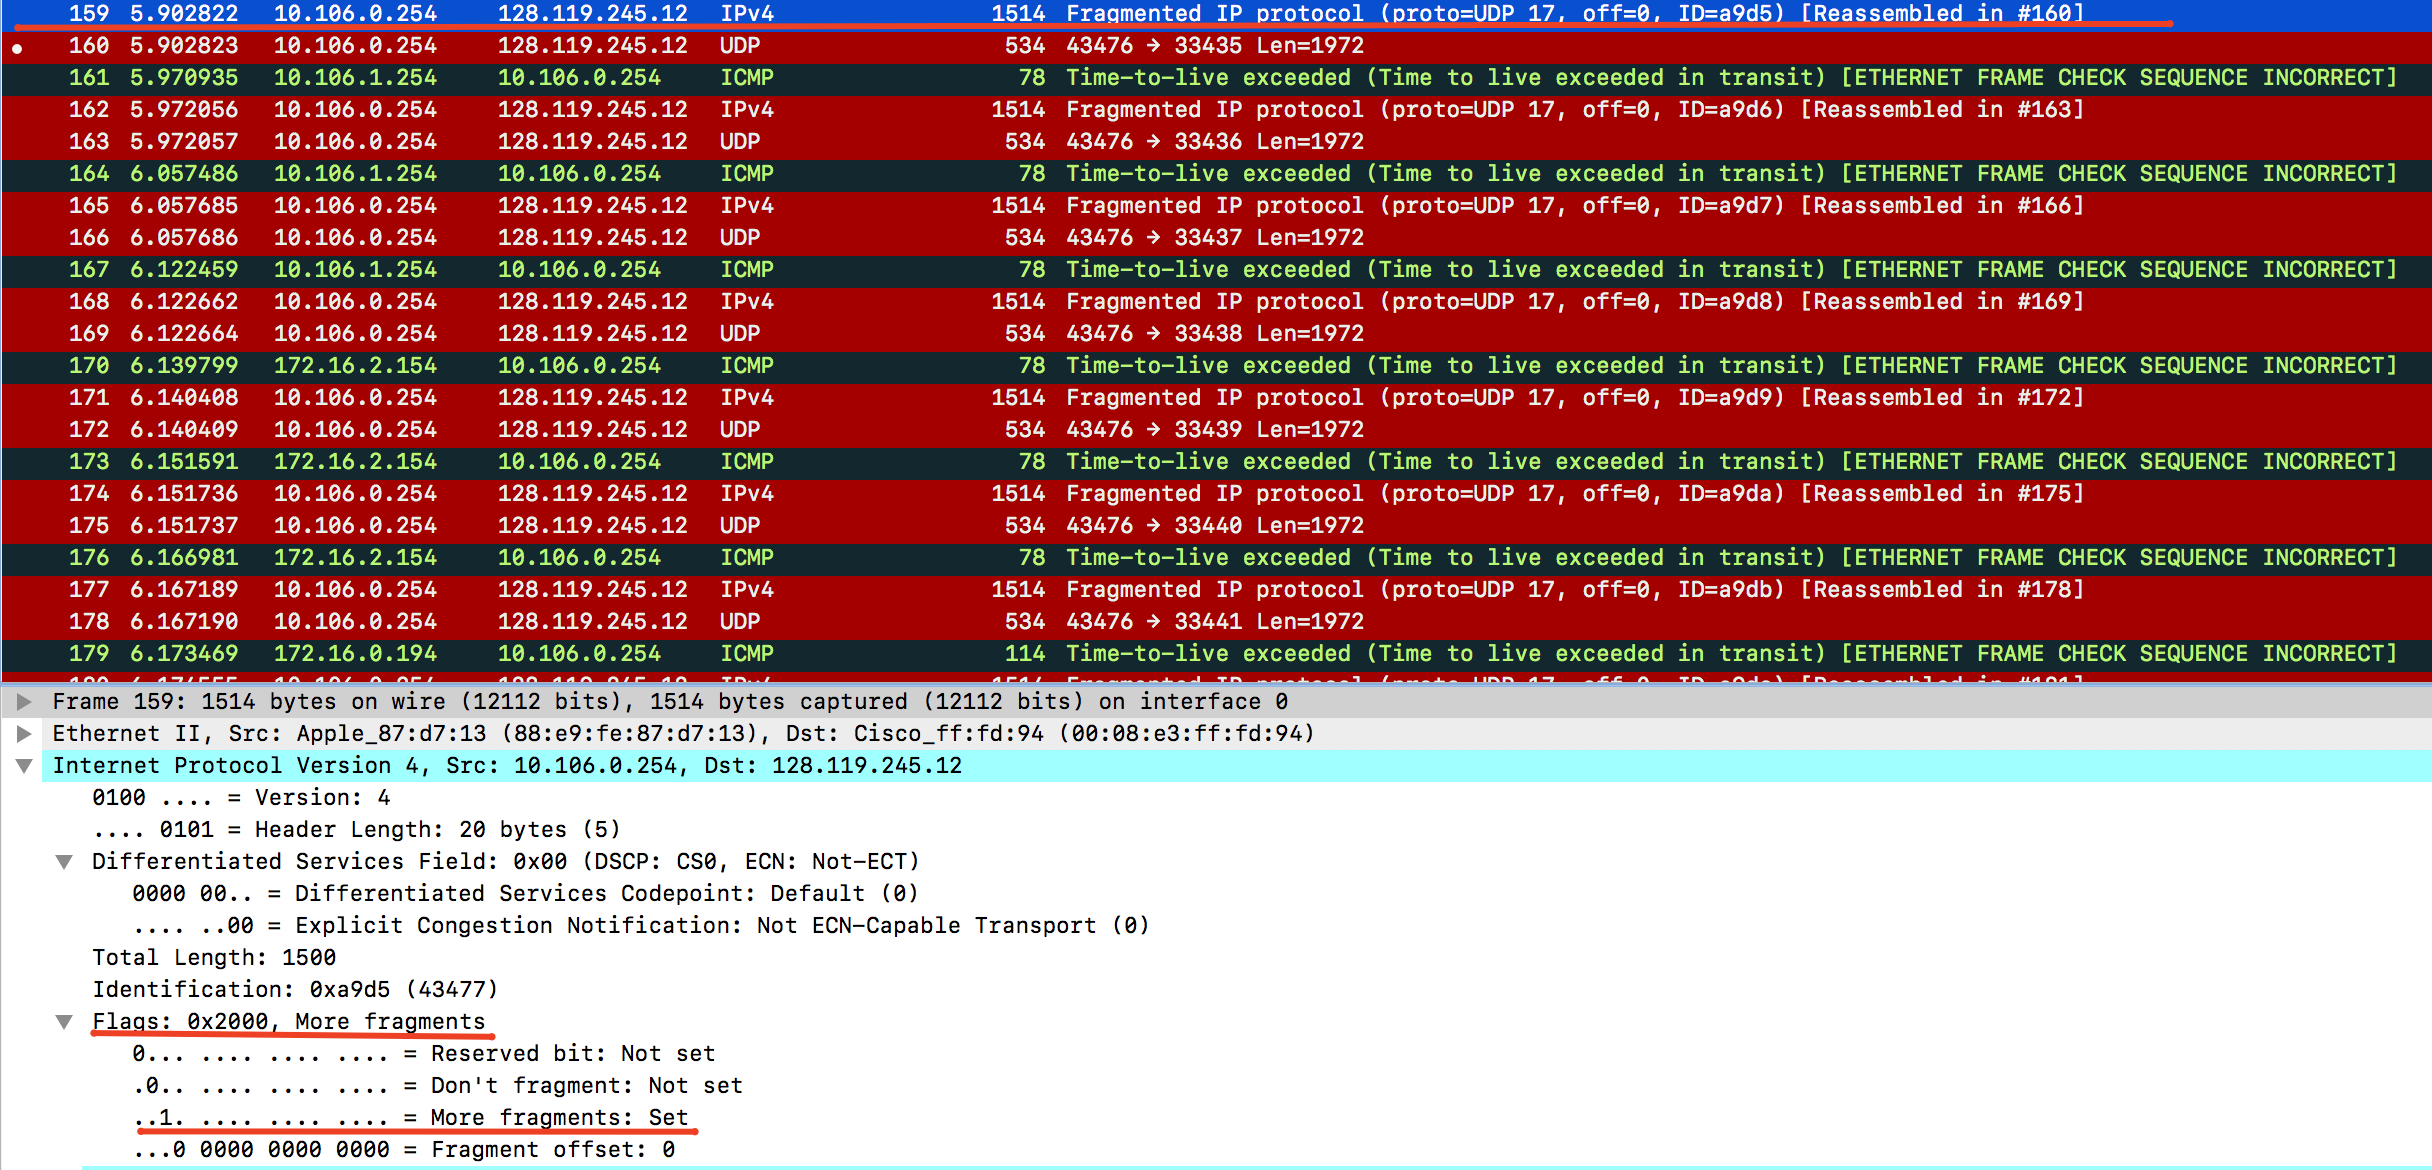
\includegraphics[scale=0.3]{images/IP10.png}
          \end{itemize}

      \item Print out the first fragment of the fragmented IP datagram.  What information in the IP header indicates that the datagram has been fragmented?  What information in the IP header indicates whether thsi is the first fragment
      versus a latter frament?  How long is this IP Datagram?
          \begin{itemize}
            \item As stated above, if the Fragment Offset is $>$ 0 or the Fragmentation Bit is set, we can tell the IP datagram has been fragmented.
            \item The 'More Fragments' offset determines the position of the current fragment in the IP datagram, because the fragment offise is zero we are working with the first fragment.
            \item The IP datagram is 1500 bytes
            \item 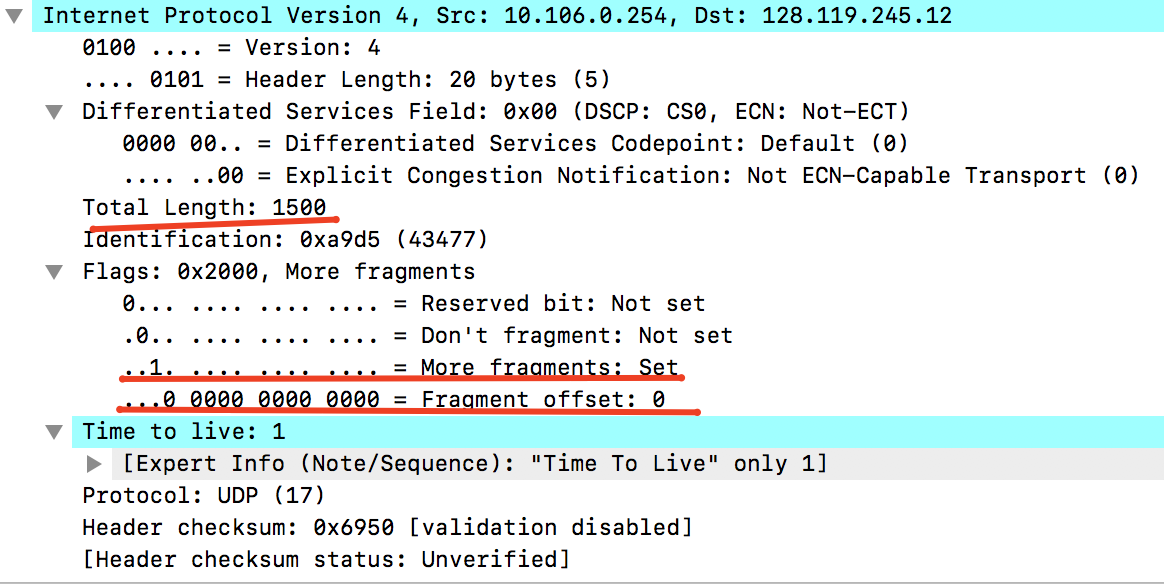
\includegraphics[scale=0.5]{images/IP11.png}

          \end{itemize}

      \item Print out the second fragment of the fragmented IP datagram.  What information in the IP header indicates that this is not the first datagram fragment.  Are there more fragments?  How can you tell?
        \begin{itemize}
          \item We know this isn't the first fragmented IP datagram because the Fragment Offset is $>$ 0.
          \item There are no more fragments following because the 'More Fragments' bit is not set.
          \item 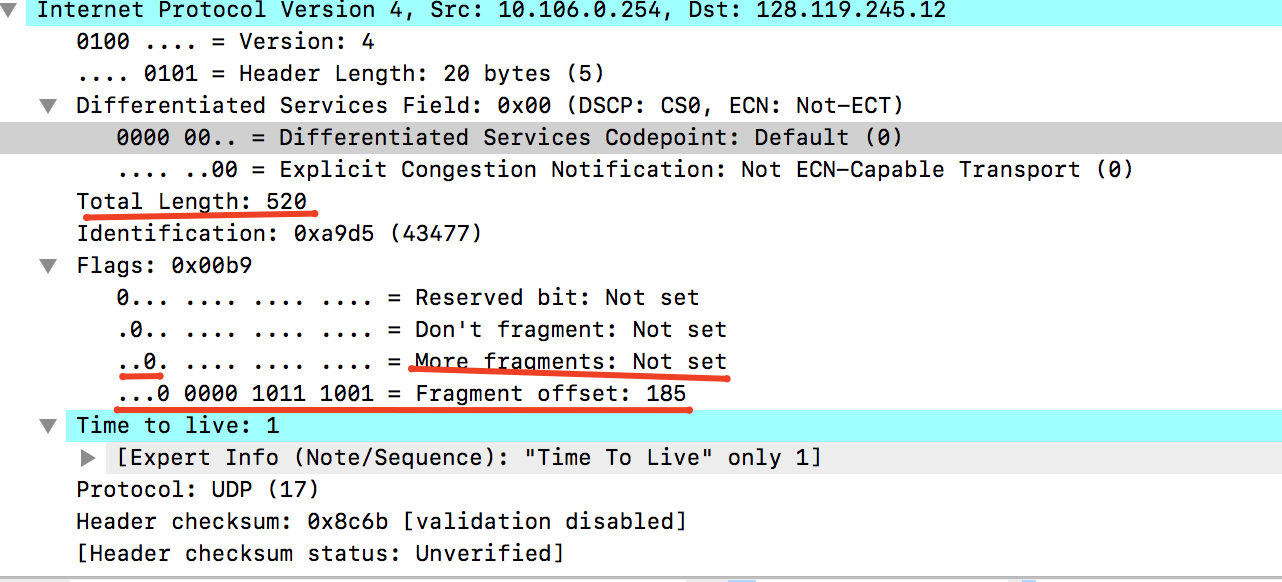
\includegraphics[scale=0.5]{images/IP12.png}
        \end{itemize}

      \item What fields change in the IP header between the first and second fragment?
        \begin{itemize}
          \item The Length of the IP datagram changes
          \item The Flags field changes, specifically the Fragmentation Bit, and the Fragmentation Offset subfields
          \item The header checksum changes
          \item Packet A:\par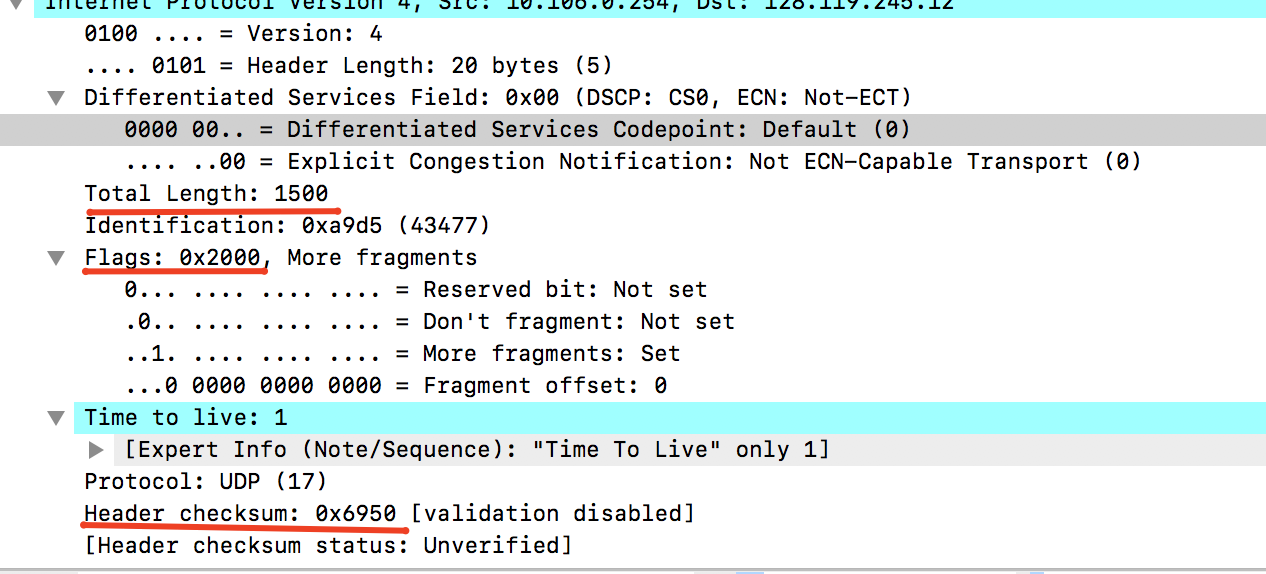
\includegraphics[scale=0.5]{images/IP13a.png}
          \item Packet B:\par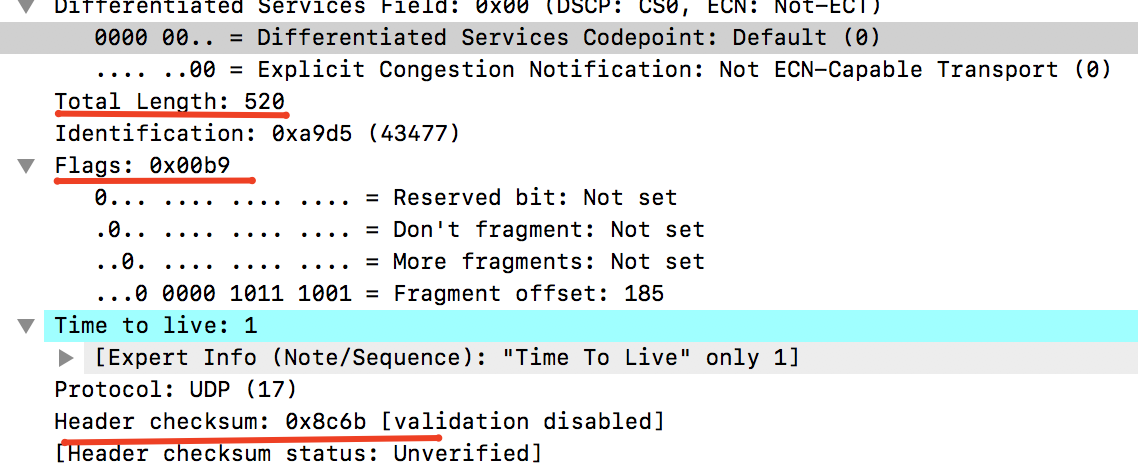
\includegraphics[scale=0.5]{images/IP13b.png}

        \end{itemize}

      \item How many Fragments were created from the original IP datagram?
        \begin{itemize}
          \item 3 Fragments were created from the original
          \item 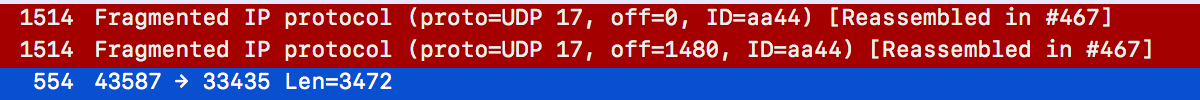
\includegraphics[scale=0.5]{images/IP14.png}
        \end{itemize}

      \item What fields change in the IP header among the fragments?
        \begin{itemize}
          \item The Length of the IP datagram changes
          \item The flags field changes, specifically the fragmentation bit, and the fragmentation offset subfields
          \item The header checksum changes
          \item Packet A:\par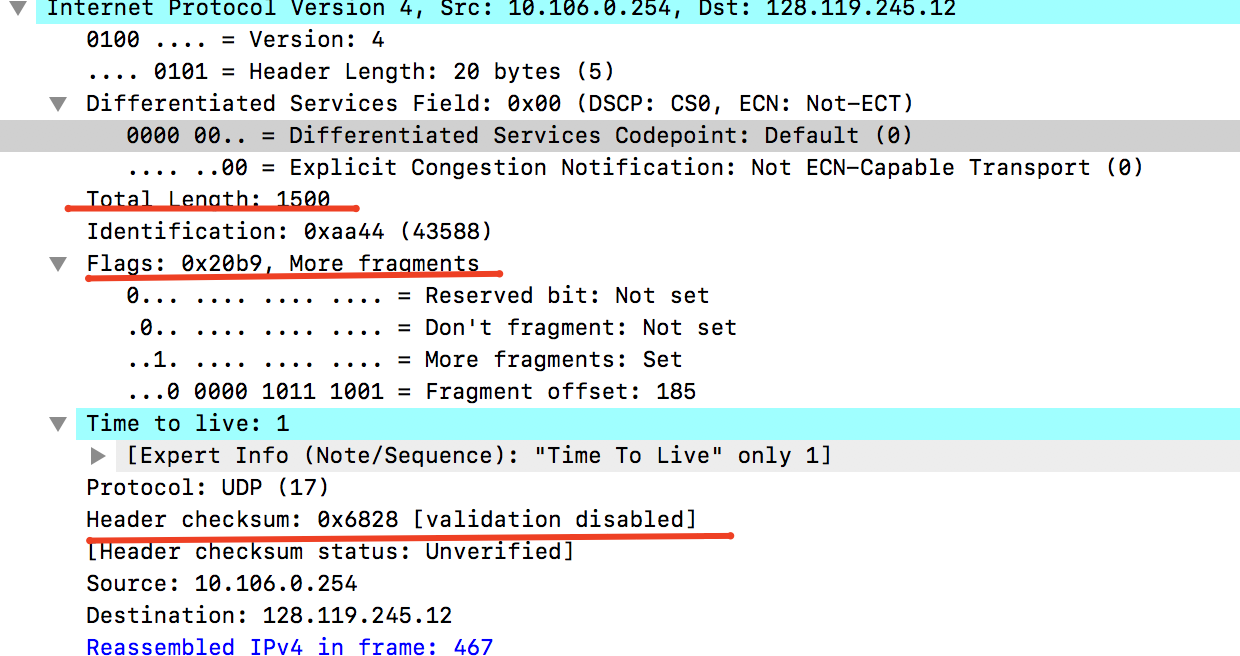
\includegraphics[scale=0.5]{images/IP15a.png}
          \item Packet B:\par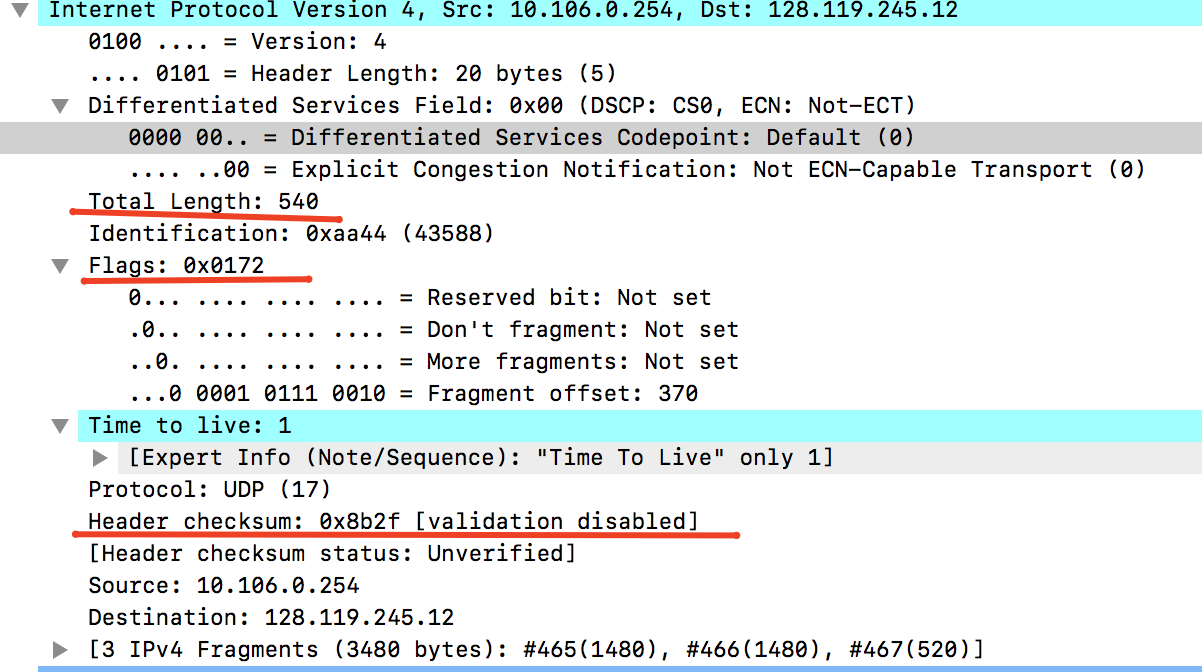
\includegraphics[scale=0.5]{images/IP15b.png}
          
        \end{itemize}
  \end{enumerate}
\end{document}
